\section{Ellipse}
\subsection{Graph}
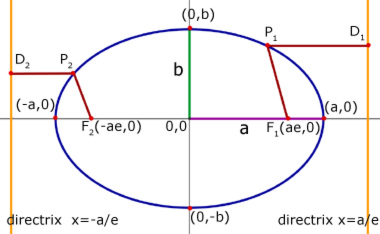
\includegraphics[width=0.4\textwidth]{ellipse.png}
\subsection{Definition}
\begin{itemize}
    \item $PF_1 + PF_2 = 2a$
    \item $\frac{\text{distance from point $P$ to a focus}}{\text{distance from the same point to the corresponding directrix}}=e=\frac{c}{a}$
\end{itemize}
\subsection{Cartesian equation}
\begin{description}
    \item[Centre $(0,0)$] $\frac{x^2}{a^2}+\frac{y^2}{b^2}=1$
    \item[Centre $(h,k)$] $\frac{(x-h)^2}{a^2}+\frac{(y-k)^2}{b^2}=1$
\end{description}
\subsection{Parametric equation}
\begin{description}
    \item[Centre $(0,0)$] $x=a\cos t$, $y=b\sin t$ ($0\leq t < 2\pi$)
    \item[Centre $(h,k)$] $x=h+a\cos t$, $y=k+b\sin t$ ($0\leq t < 2\pi$)
\end{description}
\subsection{Eccentricity}
\begin{itemize}
    \item $e=\frac{c}{a}=\sqrt{1-\frac{b^2}{a^2}}$
    \item $0<e<1$
\end{itemize}
\subsection{Directrix}
\begin{itemize}
    \item $x=h\pm \frac{a^2}{c} = h\pm\frac{a}{e}$
    \item $(h-c, 0)$ corresponds to $x=h-\frac{a}{e}$, $(h+c, 0)$ corresponds to $x=h+\frac{a}{e}$
\end{itemize}
\subsection{Tangents and normals}
\begin{itemize}
    \item Equation of tangent: $bx\cos t + ay\sin t = ab$ at $P(a\cos t, b\sin t)$
    \item Equation of normal: $ax\sin t - by\cos t=(a^2-b^2)\cos t\sin t$ at $P(a\cos t, b\sin t)$
\end{itemize}
\subsection{Chord length}
For chord $AB$ with gradient $m$:
\begin{align*}
    |AB|&=\sqrt{(1+m^2)(x_1-x_2)^2}\\
    &=\sqrt{1+m^2}\times\sqrt{(x_1+x_2)^2-4x_1x_2}
\end{align*}
\subsection{Circumference}
\begin{align*}
    C &= 4\int_{0}^{\frac{\pi}{2}}\sqrt{\left(\frac{\dx}{\dtheta}\right)^{2}+\left(\frac{\dy}{\dtheta}\right)^{2}}\dtheta\\
    &= 4a\int_{0}^{\frac{\pi}{2}}\sqrt{1-e^2\cos^2\theta}\dtheta\\
    &\approx \pi\left[3(a+b)-\sqrt{(3a+b)(3b+a)}\right]
\end{align*}

\section{Hyperbola}
\subsection{Graph}
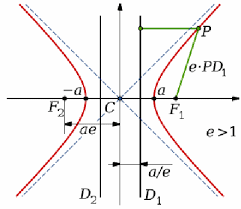
\includegraphics[width=0.4\textwidth]{hyperbola.png}
\begin{itemize}
    \item Asymptotes at $y=\pm \frac{b}{a}x$
\end{itemize}
\subsection{Definition}
\begin{itemize}
    \item $|PF_1 - PF_2| = 2a$
\end{itemize}
\subsection{Cartesian equation}
\begin{description}
    \item[Centre $(0,0)$] $\frac{x^2}{a^2}-\frac{y^2}{b^2}=1$ ($b^2=c^2-a^2$)
    \item[Centre $(h,k)$] $\frac{(x-h)^2}{a^2}-\frac{(y-k)^2}{b^2}=1$
\end{description}
\subsection{Parametric equation}
\subsubsection{Using $\sec$ and $\tan$}
\begin{description}
    \item[Centre $(0,0)$] $x=a\sec t$, $y=b\tan t$
    \item[Centre $(h,k)$] $x=h+a\sec t$, $y=k+b\tan t$
    \item[Domain] $t\neq \frac{\pi}{2}+k\pi$
\end{description}
\subsubsection{Using $\cosh$ and $\sinh$}

\begin{description}
    \item[Centre $(0,0)$] $x=\pm a\cosh t$, $y=b\sinh t$
    \item[Centre $(h,k)$] $x=h\pm a\cosh t$, $y=k+b\sinh t$
    \item[Domain] $t \in \mathbb{R}$
\end{description}
\subsection{Eccentricity}
\begin{itemize}
    \item $e=\frac{c}{a}=\sqrt{1-\frac{b^2}{a^2}}$
    \item $e>1$
\end{itemize}
\subsection{Directrix}
\begin{itemize}
    \item $x=h\pm \frac{a^2}{c} = h\pm\frac{a}{e}$
    \item $(h-c, 0)$ corresponds to $x=h+\frac{a}{e}$, $(h+c, 0)$ corresponds to $x=h-\frac{a}{e}$
\end{itemize}
\subsection{Tangents and normals}
\subsubsection{Tangent equations}
\begin{itemize}
    \item $ay\sinh t + ab = bx\cosh t$ at $P(a\cosh t, b\sinh t)$
    \item $bx\sec\theta-ay\tan\theta = ab$ at $P(a\sec\theta, b\tan\theta)$
\end{itemize}
\subsubsection{Normal equations}
\begin{itemize}
    \item $ax\sinh t + by\cosh t = (a^2+b^2)\sinh t\cosh t$ at $P(a\cosh t, b\sinh t)$
    \item $by + ax\sin\theta = (a^2+b^2)\tan\theta$ at $P(a\sec\theta, b\tan\theta)$
\end{itemize}

\section{Finding the type of the quadratic curve}
For curve $ax^2+bxy+cy^2+dx+ey+f=0$:
\begin{itemize}
    \item Find the determinant: $\Delta = b^2-4ac$
    \item $\Delta < 0$: ellipse if $a\neq c$ or $b\neq 0$, circle if $a=c$ and $b=0$
    \item $\Delta = 0$: if $a=c=0$ then a straight line, otherwise parabola
    \item $\Delta > 0$: $a=-c$ and $b=0$: intersecting lines, otherwise hyperbola
\end{itemize}